\documentclass[11pt]{article}
\usepackage{multicol}
\usepackage{ifthen}
%\usepackage{multitoc}
%\usepackage{german}
%\usepackage{bibgerm}
\usepackage{amsthm}
\usepackage{amsmath}
\usepackage{amsfonts}
\usepackage{color}
\usepackage{hyperref}
\usepackage{psfrag}
\usepackage{subfigure}
\usepackage[dvips]{epsfig}
\usepackage[dvips]{graphicx}
\usepackage[a4paper,body={148mm,240mm,nohead}]{geometry}
\usepackage[ansinew]{inputenc}
\usepackage{tikz}
\usepackage{listings}
\lstset{language=C++, basicstyle=\ttfamily,
  stringstyle=\ttfamily, commentstyle=\it, extendedchars=true}

\newif\ifpdf
\ifnum\ifx\pdfoutput\undefined0\else\pdfoutput\fi<1
\pdffalse % we are not running PDFLaTeX
\else
\pdftrue % we are running PDFLaTeX
\fi

\ifpdf
\usepackage[pdftex]{graphicx}
\else
\usepackage{graphicx}
\fi

\ifpdf
\DeclareGraphicsExtensions{.pdf, .jpg, .tif}
\else
\DeclareGraphicsExtensions{.eps, .jpg}
\fi

%\theoremstyle{plain}
\newtheorem{theorem}{Theorem}[section]
\newtheorem{lemma}[theorem]{Lemma}

\theoremstyle{definition}
\newtheorem{definition}[theorem]{Definition}
\newtheorem{class}[theorem]{Class}
\newtheorem{algorithm}[theorem]{Algorithm}
\theoremstyle{remark}
\newtheorem{remark}[theorem]{Remark}

\newcommand{\C}{\mathbb{C}}
\newcommand{\R}{\mathbb{R}}
\newcommand{\N}{\mathbb{N}}
\newcommand{\Z}{\mathbb{Z}}
\newcommand{\Q}{\mathbb{Q}}
\newcommand{\K}{\mathbb{K}}
\newcommand{\loc}{\mbox{loc}}

\title{Communication within the Iterative Solver Template Library (ISTL)\thanks{Part of the
    Distributed and Unified Numerics Environment (DUNE) which is
    available from the site
    \texttt{http://www.dune-project.org/}}}

\author{%
Markus Blatt\\
Interdisziplin�res Zentrum f�r Wissenschaftliches Rechnen,\\
Universit�t Heidelberg, Im Neuenheimer Feld 368, D-69120 Heidelberg, \\
email: \texttt{Markus.Blatt@iwr.uni-heidelberg.de}}

\date{April 27, 2005}

\begin{document}

\maketitle

\begin{abstract}
  This document describes usage and interface of the classes meant for
  setting up the communication within a parallel programm using
  ISTL. As most of the communication in distributed programm occur in
  the same pattern it is often more efficient (and of course more easy
  for the programmer) to build the communication pattern once in the
  programm and then use multiple times (e.~g. at each iteration step
  of an iterative solver).
\end{abstract}

\begin{multicols}{2}
{\small\tableofcontents}
\end{multicols}


\section{Introduction}
\label{sec:introduction}

When using the data parallel programming model a set of processes
works collectively on the same set of finite data objects. These might
be elements of a finite element grid or vector entries in a linear algebra
computation. Each process works on different partitions of the global
data. Only for this partition it computes updated values. 

In large scale parallel codes it is advisable to store the data
partition in a local data structure directly in the local memory of
the process. Due to data dependencies the process needs to access data
in the partition of other processes, too. This can either be done by
communicating these values on demand between the processes whenever
they are accessed. This results in data structures that are aware of
the data distribution. Or by augmenting the partition of the process such
that it additionally includes the data values that the other values
depend on. Note that now the partitioning is not disjoint any more but
overlapping. Of course the values other processes compute for need to
be updated using communication at so called synchronisation points of
the algorithm

In the latter case the data structures do not need to know anything
about the data distribution. 
This demands more effort from the parallel algorithm designer to make
sure that the data used for computations is valid, i.e. contains an
updated value if another process computes the data for it. Still it allows
for fewer synchronisation points in the algorithms as even in collective
operations all input data may already be updated from other processes
due to a previous operation. Between the necessary synchronisation
points one can take advantage of the fast local memory 
access.

Consider representing a random access container $x$ on a set of
processes ${\cal P}=\{0, \ldots, P-1\}$. It is represented by individual
pieces $x^p$, where $x^p$ is the piece stored on
process $p$ of the $P$ processes participating in the
calculation. Although the global representation of the container is
not available on any process, a process $p$ needs to know how the
entries of its local piece $x^p$ correspond to the entries of the
global container $x$, which would be used in a sequential program. 

\section{Communication Software Components}
\label{sec:comm-softw-comp}

From an abstract point of view a random access container $x: I
\rightarrow K$ provides a
mapping from an index set $I \subset \N_0$ onto a set of objects
$K$. Note that we do not require $I$ to be consecutive. The piece
$x_p$ of the container $x$ stored on process $p$ is a mapping $x_p:I_p
\rightarrow K$, where $I_p \subset I$. Due to efficiency the entries
of $x_p$ should be stored consecutively in memory. 
This means that for the local computation the data must be addressable
by a consecutive index starting from $0$. 

When using adaptive
discretisation methods there might be the need to reorder the indices
after adding and/or deleting some of the discretisation
points. Therefore this index does not need to be persistent
and can easily be changed. We will call this index {\em\index{local index}local index}.

For the communication phases of our algorithms these locally stored
entries must also be addressable by a global identifier. It is used to
store the received values at and to retrieve the values to be sent from the
correct local position in the consecutive  memory chunk. To ease the
addition and removal of discretisation points this global identifier has
to be persistent but does not need to be consecutive. We
will call this global identifier {\em\index{global index}global index}.

\subsection{ParallelIndexSet}
  Let $I \subset \N_0$ be an arbitrary, not necessarily consecutive,
  index set identifying all discretisation points of the computation.
  Furthermore, let 
  $$({I}_p)_{p\in {\cal P}}, \quad
  \bigcup\limits_{p \in {\cal P}} {I}_p = I$$ be an overlapping decomposition of the global index set
  $I$ into the sets of indices ${I}_p$ corresponding to the
  global indices of the values stored locally in the chunk of process $p$.

  Then the class 
  \begin{lstlisting}{}
  template<typename TG, typename TL>  class ParallelIndexSet;
  \end{lstlisting} 
  realises the one to one mapping 
  $$
  \gamma_p\::\: {I}_p \longrightarrow {I}^{\loc}_p := [0, n_p)
  $$
  of the globally unique index onto the local index. 

  The template parameter \lstinline!TG! is the type of the global
  index and
  \lstinline!TL! is the type of the local index. The only prerequisite
  of \lstinline!TG! is that objects of this type are comparable using
  the less-than-operator \lstinline!<!. Not that this prerequisite
  still allows attaching further 
  information to the global index or even using this information as
  the global index. The type \lstinline!TL! has to
  be convertible to  \lstinline!std::size_t! as it is used to address array
  elements. 

  The pairs of global and local indices are
  ordered by ascending global index. It is possible to access the pairs via
\lstinline!operator[](TG& global)! in $log(n)$ time, where $n$ is the
number of pairs in the set. In an efficient code it is advisable to
access the index pairs using the provided iterators over the index pairs.

Due to the ordering, the index set can only be changed, i.e. index pairs
added or deleted, in a special resize phase. By calling the functions
\lstinline!beginResize()! and \lstinline!endResize()! the programmer
indicates that the resize phase starts and ends, respectively. During
the call of \lstinline!endResize()! the deleted indices will be
removed and the added index pairs will be sorted and merged with the existing
ones.

\subsection{ParallelLocalIndex}
When dealing with overlapping index sets in distributed computing
there often is the need to distinguish different partitions of an index
set.%, e.g. $I_i$ and $\tilde{I}_i\setminus I_i$ as introduced in Section \ref{sec:domain_decomposition}.

This is accomplished by using the class
\begin{lstlisting}{}
  template<typename TA> class ParallelLocalIndex;
\end{lstlisting}
as the type for the local index of class \lstinline!ParallelIndexSet!.
Here the template parameter \lstinline!TA! is the type of the
attributes used, e.g. an enumeration \lstinline!Flags! defined by
\begin{lstlisting}
  enum Flags {owner, ghost};
\end{lstlisting}
where 
\lstinline!owner! marks the indices $k \in I_p$ owned by process
$p$ and \lstinline!ghost! the indices $k\not\in I_p$ owned
by other processes.

As an example let us look at an array distributed between two
processes. In Figure \ref{fig:redistarray} one can see the array
$a$ as it appears in a sequential program. Below there are two
different distributions of that array. The local views $s_0$ and
$s_1$ are the parts process $0$ and $1$ store in the case that $a$ is
divided into two 
blocks. The local views $t_0$ and $t_1$  are the parts of $a$ that
process $0$ and $1$ store in the case that $a$ is divided into 4
blocks and process 
$0$ stores the first and third block and process $1$ the second and
fourth block. The decompositions have an overlap of one and the indices have
the attributes \lstinline!owner! and \lstinline!ghost! visualised by
white and shaded cells, respectively.
The index sets $I_s$ and $I_t$ corresponding to the decompositions $s_p$
and $t_p$, $p \in \{0,1\}$, are shown in Figure \ref{fig:redistindex} as sets of triples
$(g,l,a)$. Here $g$ is the global index, $l$ is the local index and
$a$ is the attribute (either o for \lstinline!owner! or {g}
for \lstinline!ghost!).
\begin{figure}%[b]
  \centering
  \psfrag{Is}{$I_s$}
  \psfrag{It}{$I_t$}
  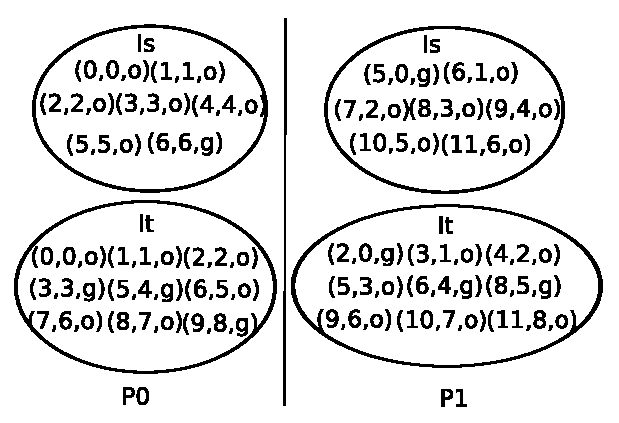
\epsfig{file=figures/distindex.eps,width=.5\textwidth}
  \caption{Index sets for array redistribution}
  \label{fig:redistindex}
\end{figure}
\begin{figure*}%[b]
  \tikzset{
    box/.style={
      draw,
      shape=rectangle,
      minimum width=1.5em,
      minimum height=1.5em,
      anchor=base,
      inner sep=0pt,
    },
    overlap/.style={fill=black!25!white},
  }
  \newcommand{\interior}[1]{%
    \tikz[baseline={(0,0)}]\node[box]{#1};%
  }
  \newcommand{\overlap}[1]{%
    \tikz[baseline={(0,0)}]\node[box,overlap]{#1};%
  }
  \def\mc{\multicolumn}%
  \newcommand{\leader}[1]{\makebox[2em][r]{#1 }}%
  \renewcommand{\arraystretch}{2}%
  \centering
  \begin{tabular}{r|l}
    \mc2c{global array} \\
    \mc2c{\leader{a:}%
            \foreach\i in {0,...,11} {\interior{\i}}} \\
    \mc2c{local views} \\
    \leader{$s_0$:}%
      \foreach\i in {0,...,5}  {\interior{\i}}%
      \foreach\i in {6}        {\overlap {\i}} &
    \leader{$s_1$:}%
      \foreach\i in {5}        {\overlap {\i}}%
      \foreach\i in {6,...,11} {\interior{\i}} \\
    \leader{$t_0$:}%
      \foreach\i in {0,1,2}    {\interior{\i}}%
      \foreach\i in {3,5}      {\overlap {\i}}%
      \foreach\i in {6,7,8}    {\interior{\i}}%
      \foreach\i in {9}        {\overlap {\i}} &
    \leader{$t_1$:}%
      \foreach\i in {2}        {\overlap {\i}}%
      \foreach\i in {3,4,5}    {\interior{\i}}%
      \foreach\i in {6,8}      {\overlap {\i}}%
      \foreach\i in {9,10,11}  {\interior{\i}} \\
    \mc1c{P0} & \mc1{|c}{P1} \\
  \end{tabular}
  \caption{Redistributed array}
  \label{fig:redistarray}
\end{figure*}

The following code snippet demonstrates how to set up the index set
$I_s$ on process $0$:
\lstinputlisting[linerange={53-57,59-61,67-67}]{poosc08_test.cc}
\subsection{Remote Indices}
\label{sec:remote-indices}

To set up communication between the processes every process needs to
know which indices are also known to other processes and which
attributes are attached to them on the remote side.
There are scenarios where data is exchanged between different
index sets, e.g. if the data is agglomerated on lesser processes or
redistributed. Therefore communication is allowed to occur between different
decompositions of the same index set.


Let $I \subset \N$ be the global index set and 
$$
(I^s_p)_{p\in{\cal P}},\quad \bigcup_{p\in{\cal P}} I^s_p = I,\quad
\text{ and } \quad
(I^t_p)_{p\in{\cal P}}, \quad\bigcup_{p\in{\cal P}} I^t_p = I
$$ be two overlapping
decompositions of the same index set $I$. Then an instance of class
\lstinline!RemoteIndices! on process $p \in {\cal P}$
stores the sets of triples
\begin{equation}
  \label{eq:ri_s_set}
  \begin{split}
  r_{p \rightarrow q}^{s} = \{ (g,(l,a),b) \,|\, g \in I^s_q \wedge g \in I_p^t,
l=\gamma_p^s(g),  a = \alpha_p^s(l), b =
\alpha_q^t(\gamma_q^t(g))\}
\end{split}
\end{equation}
and
\begin{equation}
  \label{eq:ri_t_set}
  \begin{split}
  r_{p \rightarrow q}^{t} = \{ (g,(l,a),b) \,|\, g \in I^s_q \wedge g \in I_p^t,
  l=\gamma_p^t(g), a = \alpha_p^t(l), b =
  \alpha_p^s(\gamma_p^s(g))\}\,,
  \end{split}
\end{equation}
for all $q\in{\cal P}$.
Here $\alpha^s_p$ and $\alpha^t_p$ denote the mapping of local
indices on process $p$ onto attributes for the index set $I^s_p$ and
$I^t_p$ as realised by \lstinline!ParallelLocalIndex!. 
Note that the sets $r_{p \rightarrow q}^{s}$ and $r_{p \rightarrow
  q}^{t}$ will only be nonempty if the processes $p$ and $q$ manage
overlapping index sets.

For our example in Figure \ref{fig:redistarray} and Figure
\ref{fig:redistindex} the interface between $I_s$ and $I_t$ on process
$0$ is:
\begin{align*}
  r_{0\rightarrow 0}^{s} = \{&(0,(0,o),o), (1,(1,o),o), (2,(2,o),o),
  (3,(3,o),g), (5,(5,o),g), (6,(6,g),o)\}\\
  r_{0\rightarrow 0}^{t} = \{&(0,(0,o),o), (1,(1,o),o), (2,(2,o),o),
  (3,(3,g),o), (5,(4,g),o), (6,(5,o),g)\}\\
  r_{0\rightarrow 1}^{s} = \{&(2(2,o),g), (3,(3,o),o), (4,(4,o),o),
  (5,(5,o),o), (6,(6,g),g)\}\\
  r_{0\rightarrow 1}^{t} = \{&(5,(4,g),g), (6,(5,o),o), (7,(6,o),o),
  (8,(7,o),o), (9,(8,g),o)\}
\end{align*}
This information can either be calculated automatically by
communicating all indices in a ring or set up by hand if the user has
this information available. Assuming that \lstinline!sis! is the index set
$I_s$ and \lstinline!tis! the index set $I_t$ set up as described in
the previous subsection  and \lstinline!comm! is an MPI communicator
then the simple call
\lstinputlisting[linerange={83-84}]{poosc08_test.cc}
on all processes automatically calculates this information and
stores it in \lstinline!riRedist!. For a
parallel calculation on the local views $s_0$ and $s_1$ calling
\lstinputlisting[linerange={86-87}]{poosc08_test.cc}
on all processes builds the necessary information in \lstinline!riS!.

\subsection{Communication Interface}
\label{sec:comm-interf}

With the information provided by class \lstinline!RemoteIndices! the
user can set up arbitrary communication interfaces. These interfaces
are realised in \lstinline!template<typename T> class Interface!,
where the template parameter \lstinline!T! is the custom type of the
\lstinline!ParallelIndexSet! representing the index sets. 
Using the attributes attached to the indices by
\lstinline!ParallelLocalIndex! the user can select subsets of the
indices for exchanging data, e.g. send data from indices marked
as \lstinline!owner! to indices marked as \lstinline!ghost!.

Basically the interface on process $p$ manages two sets for each
process $q$ it shares common indices with:

$$
i_{p\rightarrow q}^{s} = \{ l | (g,(l,a),b) \in r_{p\rightarrow q}^{s} |
a \in A_s \wedge b \in A_t\}
$$
and
$$
i_{p\rightarrow q}^{t} = \{ l | (g, (l,a), b) \in r_{p\rightarrow q}^{t} |
a \in A_t \wedge b \in A_s\}\,,
$$
where $A_s$ and $A_t$ are the attributes marking the indices where the
source and target of the communication will be, respectively.

In our example these sets on process $0$ will be stored for
communication if $A_s=\{o\}$ and $A_t=\{o, g\}$:
\begin{align*}
  i_{0\rightarrow 0}^{s} =  \{0, 1, 3, 5\}\quad & \quad
  i_{0\rightarrow 0}^{t} =  \{0, 1, 3, 4\}\\
  i_{0\rightarrow 1}^{s} =  \{2, 3, 4, 5\}\quad & \quad
  i_{0\rightarrow 1}^{t} =  \{5, 6, 7, 8\}\,.
\end{align*}

The following code snippet would build the interface above in
\lstinline!infRedist! as well as the interface \lstinline!infS!
to communicate between
indices marked as \lstinline!owner! and \lstinline!ghost! on the local
array views $s_0$ and $s_1$:
\lstinputlisting[linerange={89-97}]{poosc08_test.cc}

\subsection{Communicator}
\label{sec:communicator}

Using the classes from the previous sections all information about the
communication is available and we are set to communicate data values
of arbitrary
container types. The only prerequisite for the container type is that
its values are addressable via \lstinline!operator[](size_t index)!.
This should be safe to assume. 

An important feature of our communicators is that we are not only able to
send one data item per index, but also different numbers of data
elements (of the same type) for each index. This is
supported in a generic way by the traits class 
\lstinline!template<class V> struct CommPolicy! 
describing the container type \lstinline!V!. The 
\lstinline!typedef IndexedType! is the atomic type to be communicated and
\lstinline!typedef IndexedTypeFlag! is either \lstinline!SizeOne! if
there is only one data item per index or \lstinline!VariableSize! if the
number of data items per index is variable.

The default implementation works for all
array-like containers which provide only one data item per index. For all
other containers the user has to provide its own custom
specialisation. 
%For the vector classes of ISTL (up to two block levels)
%those specialisations are already implemented.

The class \lstinline!template<class T> class BufferedCommunicator!
performs the 
actual communication. The template parameter \lstinline!T! describes
the type of the parallel index set.
It uses the information about the communication interface provided by
an object of class \lstinline!Interface! to set up communication
buffers for a container containing a specific data type. It is also
responsible for gathering the data before and scattering the data
after the communication step. The strict separation of the interface
description from the actual buffering and communication allows for
reusing the interface information with various different container and
data types.

Before the communication can start one has to call the
\lstinline!build! method with the data source and target containers as
well as the communication interface as arguments. Assuming
\lstinline!s! and \lstinline!t! as arrays $s_i$ and $t_i$,
respectively, then
\lstinputlisting[linerange=103-106]{poosc08_test.cc}
demonstrates how to set up the communicator \lstinline!bCommRedist! for the array
redistribution and \lstinline!bComm! for a parallel calculation on the
local views $s_i$. The
\lstinline!build! function
calculates the size of the messages to send to other processes and
allocates buffers for the send and receive actions. The
representatives \lstinline!s! and \lstinline!t! are
needed to get the number of data values at each index in the case of
variable numbers of data items per index. Note that, due to the generic
programming techniques used, the compiler knows if the number of data
points is constant for each index and will apply a specialised
algorithm for calculating the message size without querying neither
\lstinline!s! nor  \lstinline!t!. Clean up of allocated
resources is done either by calling the method \lstinline!free()! or
automatically in the destructor.

The actual communication takes place if one of the methods
\lstinline!forward!
and \lstinline!backward! is called. In our case in
\lstinline!bCommRedist! the \lstinline!forward! method
sends data from the local views $s_i$ to the local views $t_i$
according to the interface information and the \lstinline!backward!
method in the opposite direction. 

The following code snippet first redistributes the local views $s_i$
of the global array to the local views $t_i$ and
performs some calculation on this representation. Afterwards the
result is communicated backwards.
\lstinputlisting[linerange=110-113]{poosc08_test.cc}

Note that both methods have a different template parameter, either
\lstinline!CopyData! or \lstinline!AddData!. These are policies for
gathering and scattering the data items. The former just copies
the data from and to the location. The latter copies from the source
location but adds the received data items to the target
entries. Assuming our data is stored in simple C-arrays
\lstinline!AddData! could be implemented like this:

\lstinputlisting[linerange=16-27]{poosc08_test.cc}

Note that arbitrary
manipulations can be applied to the communicated data in both methods.

For containers with multiple data items associated with one index
the methods \lstinline!gather! and \lstinline!scatter! must have an additional
integer argument specifying the sub-index. 

\section{Collective Communication}
\label{sec:collective-communication}

While communicating entries of array-like structures is a prominent
task in scientific computing  codes one must not neglect
collective communication operations, like gathering and scattering data
 from and to all processes, respectively, or waiting for other processes. An
abstraction for these operations is crucial for decoupling the
communication from the parallel programming paradigm used.

Therefore we designed 
\lstinline!template<class T> class CollectiveCommunication! which provides
information of the underlying parallel programming paradigm as well as
the collective communication operations as known from MPI. See Table
\ref{tab:col-comm} for a list of all functions. 

\begin{table*}%[b]
  \centering
  \begin{tabular}{p{.5\textwidth}|p{.4\textwidth}}
    Function&Description\\\hline\hline
    \lstinline!int rank()!&Get the rank of the process\\
    \lstinline!int size()!&Get the number of processes\\
    \lstinline!template<typename T> T sum (T& in)!& Compute global
    sum\\
    \lstinline!template<typename T> T prod (T& in)!&Compute global
    product\\
    \lstinline!template<typename T> T min (T& in)!&Compute global minimum\\
    \lstinline!template<typename T> T max (T& in)!&Compute global
    maximum\\
    \lstinline!void barrier()!& Wait for all processes.\\
    \lstinline!template<typename T> int broadcast (T* inout, int len, int root)! 
& Broadcast an array from root to all other processes\\
\lstinline!template<typename T> int gather (T* in, T* out, int len, int root)!&
Gather arrays at a root process\\
\lstinline!template<typename BinaryFunction, typename Type> int allreduce(Type* in, Type* out, int len)!&
Combine values from all processes on all processes. Combine function
is given with \lstinline!BinaryFunction!
  \end{tabular}
  \caption{Collective Communication Functions}
  \label{tab:col-comm}
\end{table*}

Currently there is a default implementation for sequential programs
as well as a specialisation working with MPI. This approach allows for
running parallel programs sequentially without any parallel overhead
simply by choosing the sequential specialisation at compile time.
Note that the interface is far more convenient to use than the C++
interface of MPI. The latter is a simple wrapper around the C
implementation without taking advantage of the power of generic programming.


The collective communication classes were developed before the release
of Boost.MPI \cite{boost_mpi}. In contrast to Boost.MPI it was never
meant as a full generic implementation of all MPI functions. Instead it
is restricted to the most basic subset of collective operations needed
to implement finite element methods and iterative solver using the
previously described components. This lean interface should make it
possible to easily port this approach to
thread based parallelisation as well as other parallelisation
paradigms. This would allow code to easily switch between different paradigms


\bibliographystyle{plainnat}
\bibliography{communication}
\end{document}
%%% Local Variables: 
%%% mode: latex
%%% TeX-master: t
%%% End: 
